\chapter{Analysis overview}
\label{ch:an_overview}

In 2012, CMS~\cite{HiggsCMS} and
ATLAS~\cite{HiggsAtlas} collaborations officially discovered a Higgs-like particle and with that breakthrough the picture of the
SM \cite{Salam:1961en,Glashow:1961tr,Weinberg:1967tq}
of the particle physics has been completed. 
Most of the basic properties of the Higgs
boson have been measured. 
However, it remains difficult to distinguish several processes with very low
cross sections from the
irreducible SM background processes with a similar signature. 
One such important but rare process is a double Higgs (HH) boson
production. HH directly relates to the Higgs boson self-coupling, and thus,  
has an access to the shape of the Higgs boson potential. In the SM, HH
production is a non-resonant process with a cross section of $\sigma$
=  fb~\cite{HHXsec} at $\sqrt{s}=13$~TeV. 

Several Beyond the Standard
Model (BSM) theories and models, such as supersymmetry, composite Higgs, Warped Extra Dimensions (WED)~\cite{Dolan:2012ac, Huang:2017nnw, Kanemura:2016tan, Oliveira:2014kla, WED}, predict scenarios when the double Higgs boson
cross section is significantly increased and may be observed with the current data.
There may be two different types of the BSM HH production: a non-resonant production,
introducing BSM terms to the SM lagrangian or a resonant production,
in which the process is mediated by a narrow width heavy mass resonance that subsequently would decay to SM Higgs bosons. 
~\cite{WED}. %%\newline
\vspace{1em} % adds some space


In this analysis through the gluon fusion mechanism a heavy narrow
resonance, such as RS1 KK graviton or RS1 radion ("graviton" or "radion" later in the text) \cite{BG1,BG2,BG3} is produced. It decays to two Higgs bosons, which further decay to the bb pair (the first Higgs boson) and the ZZ/WW pair (the other Higgs boson). 
The analysis covers masses of graviton/radion from 250 GeV to 1000 GeV. Since no evidence of the signal has been reported by the previous HH analyses, we proceed directly to setting 95 \% upper confidence
limits on the production of the graviton with a subsequent
decay to Higgs bosons times the branching ratios of the Higgs
boson decaying to a pair of b quarks and the other Higgs boson to two
leptons and two neutrinos respectively (Fig. ~\ref{fig:BGtoHH}). We observe no deviation with the given data and
evaluated uncertainties, the results are compatible with the Standard
Model.


\begin{figure}[!htb]%hbpt?
  \begin{center}
    %\raisebox{0.17\height}
    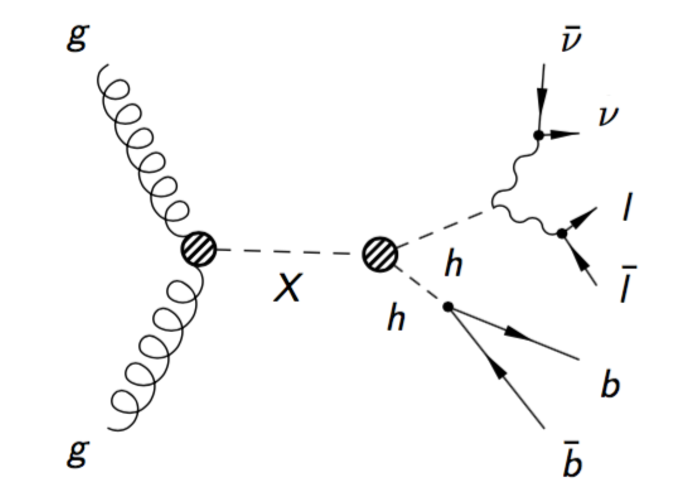
\includegraphics[width=0.45\textwidth]{BGtoHH.pdf}
    \caption{ The Feynman diagram of the graviton/radion production with the subsequent decay to HH. HH system decays to a pair of b quarks and Z bosons. Shown is 2 b quarks, 2 leptons, and 2 neutrinos final state.
    }
    \label{fig:BGtoHH}
  \end{center}
\end{figure}


\section{Analysis Strategy}

The analysis is based on ntuples and object selection from the approved VHbb sister analysis~\cite{VHbb_inspire}. Leptons, b jets, and the missing transverse energy (MET) are reconstructed using the standard CMS procedures~\cite{CMSreco} and the Particle Flow (PF) algorithm~\cite{PFalgo}. b-jets are identified using the Combined MVA v2 (CMVA) algorithm~\cite{BTagtwiki}. Then, on shell Z boson candidates are selected of dilepton pairs of the same flavour with a net charge zero for a pair. Higgs boson candidate decaying to b quarks (Hbb) is reconstructed as a pair of b jets with the highest CMVA output value. Finally, double Higgs boson pseudo-transverse mass, which is used in the shape analysis to extract limits, is constructed computing the transverse mass of the sum of the Lorentz vectors of the two leptons forming the on-shell Z, MET, and a pair of the b jets forming the \HBB. Additionally, a cut on the missing transverse energy is introduced to preserves the orthogonality with the existing HIG-18-013 ``2b 2l 2q'' analysis, which also works with the $bbZZ$ decays. In a similar fashion, the cut on the Z mass ($m_Z > 76$ GeV) is used to orthogonalise the analysis with respect to the HH phase space used in the legacy $bbWW$ analysis where the final signature is identical to ours. Lastly, the cut on the BDT is used to reduce the background contamination in the signal region.

Main backgrounds are \ttbar and Drell-Yan in association with jets. To determine their normalization, we construct two dedicated control region, which are correspondingly \ttbar and Drell-Yan dominated. Then, during the the simultaneous fit of signal region (SR), as well as control region \ttbar (CRTT), and control region Drell-Yan (CRDY), we obtain rates for these processes. Others, minor backgrounds, are single top production, diboson samples (WW, WZ, ZZ), and ZH production and are determined from the Monte Carlo (MC) simulation. 
%We assign systematics uncertainties on the QCD scale corresponding to each process. Also uncertainty associated with the imperfect knowledge of the single top cross section is added.

In the next chapters we will discuss all of the aspects of the analysis in details starting with the chapter on Data. 
